\documentclass[a4paper,10pt]{article}
\usepackage[utf8]{inputenc}
\usepackage{geometry} %自定义布局
\usepackage{multicol} %双栏
\usepackage{graphicx} %图像
\usepackage{amsmath} % 数学单位等等
\usepackage[runin]{abstract} %摘要修改 摘要标题添加到摘要正文段前
\usepackage{booktabs}%三线格
\usepackage{float}%浮点
\usepackage{cite}%引用
\usepackage{pdfpages}%pdf合并
\geometry{a4paper,left=1.6cm,right=1.6cm,top=2cm,bottom=2cm}
\graphicspath{{picture/},{pics/}}
%opening
\title{\bfseries The Analysis of Mutagenesis Results of WP2 Bacteria By MMS and UV light}
%%%标题加粗
\author{Kangyao Ma}
\date{}


\begin{document}


\maketitle


\setlength{\absleftindent}{0pt}
\setlength{\absrightindent}{0pt}
\setlength{\abstitleskip}{-1.5em}
\abslabeldelim{:}
\renewcommand{\abstractnamefont}{\itshape\bfseries}
\renewcommand{\absnamepos}{flushleft}
\begin{abstract}
\textit{\small The WP2 assay, also known as the tryptophan reverse mutation assay, detects the production of additional revertants induced from tryptophan auxotrophs, indicating a positive mutagenic effect. This experiment aimed to investigate bacterial mutagenesis using the chemical methyl methanesulfonate (MMS) and ultraviolet (UV) light to assess their impact on cells. The experimental approach involved determining the appropriate E. coli concentration based on the OD value, applying MMS and UV mutagenesis treatments to each plate, estimating the number of viable cells through serial dilution, and setting up different control groups to calculate spontaneous mutations and assess the degree of mutation induction.The results indicate that both MMS and UV radiation have mutagenic effects on E. coli auxotrophs. However, these effects exhibit a non-linear relationship with MMS concentration. Additionally, a relatively short UV irradiation time induces noticeable mutagenesis, while excessively long exposure may lead to a reduction in bacterial colonies due to the damaging effects of prolonged UV exposure. The adverse cytotoxicity of MMS appears to obscure mutagenic effects in treatment plate assays.}
\end{abstract}


\hrule


\begin{multicols}{2}
\section{Introduction}


Mutagens are substances that can cause sudden or fundamental changes in an organism's genetic material, leading to genetic mutations or chromosome aberrations beyond natural levels \cite{chaudhary2019mutagenesis}. The genetic toxicity test using Escherichia coli WP2 has been widely employed in assessing the safety of food, medicine, cosmetics, and the environment due to its high sensitivity to various mutagens \cite{brusick1980evaluation}. Escherichia coli tryptophan auxotrophic strains, such as WP2 $trp^-$, cannot synthesize tryptophan due to a mutation in the trpE65 allele, which contains an ochre stop codon (TAA) instead of a glutamine codon (CAA)\cite{ohta2002characterization}.

This assay is valuable for mutagen screening because it allows only revertant bacteria to grow on medium lacking tryptophan. Spontaneous reversion mutations occur at a low frequency. In the presence of a mutagenic substance, auxotrophic bacteria may revert to prototrophic type through two main mechanisms. The first involves a mutation within the original ochre codon, changing TAA to glutamine (CAA), glutamic acid (GAA), leucine (TTA), serine (TCA). Alternatively, a second location mutation may occur involving an ochre suppressor mutation at anticodon sites in tRNA genes.

Prolonged UV exposure would kill too many bacteria to be detected, given UV light's disinfection function. However, defining what constitutes prolonged exposure is challenging \cite{grzesiuk1994frequency}\cite{sobol2002mutations}. For instance, while 20 seconds of exposure may be suitable for inducing mutations, a 40-second period is not appropriate. The specific trends within the 20-second interval are not characterized. Therefore, additional experimental groups with smaller exposure intervals are required to comprehensively study UV mutagenesis \cite{brash1982uv}\cite{ikehata2011mechanisms}.

Therefore, in addition to spontaneously developed revertants, there will be additional revertants capable of growing and forming colonies on tryptophan-limited medium in the presence of a mutagen, indicating a positive result. The E. coli WP2 strain is a commonly used genetic marker in radiation studies, DNA repair mechanism analysis, and mutagenesis research. In this experiment, we aim to investigate chemical mutagenesis using methyl methanesulfonate (MMS) and UV light mutagenesis using the WP2 assay with an E. coli trp- strain under different conditions. Specific control groups are included for estimating viable cell counts and determining spontaneous mutation rates.


\section{Material and Method}


\begin{center}
{\footnotesize Table 1. Materials needed for this experiment}
\begin{table}[H]
\footnotesize
\begin{tabular}{cc}
\toprule [1pt]
\textbf{Cells Preparation}&\textbf{Explanation}\\
\hline
E. coli $Trp^-$ strain&\\
Liquid growth medium&\\
PBS, pH 7.4& \textgreater25 mL\\
1.5 mL microcentrifuge tubes&1\\
\hline
\textbf{Serial dilutions}&\\
\hline
E. coli $Trp^-$ culture suspension ($10^8$cells/mL)&0.1mL\\
1.5 mL microcentrifuge tubes&6\\
PBS&5.5\\
\hline
\textbf{Cell mutagenesis}&\\
\hline
SA1 plate (0.25 \textmu g/mL tryptophan)&2\\
SA2 plate (1 \textmu g/mL tryptophan)&6\\
SA3 plate (0 \textmu g/mL tryptophan)&2\\
NA plate (plenty of tryptophan)&2\\
E. coli $Trp^+$ culture suspension&0.1mL\\
E. coli $Trp^-$ culture suspension ($10^8$cells/mL)&1mL\\
E. coli $Trp^-$ culture suspension ($10^3$cells/mL)&0.1mL\\
E. coli $Trp^-$ culture suspension ($10^2$cells/mL)&0.1mL\\
1\% MMS&50\textmu L\\
2\% MMS&25\textmu L\\
Sterile water&25\textmu L\\
Sterile inoculating loop&1\\
Sterile beads&\\
\bottomrule [1.5pt]
\end{tabular}
\end{table}
\end{center}


\subsection{Cells Preparation}
Inoculate Escherichia coli into a liquid culture medium. After 2.5 hours, begin monitoring the optical density at 600 nm (OD600) of the liquid growth medium as a control, checking every 30 to 15 minutes until the value reaches 0.30-0.35, indicating a concentration of approximately $2\times 10^8$ E. coli cells/mL in the mid-logarithmic phase. Subsequently, wash the bacteria by removing the growth medium and centrifuging at 10,000 rpm for 10 minutes. Following removal of the supernatant, resuspend the pellet in 15-20 mL of phosphate-buffered saline (PBS) at pH 7.4. Centrifuge again at 10,000 rpm for 10 minutes, then resuspend the pellet in 4 mL of PBS and use PBS as a blank to check the OD600. Distribute cells into multiple 1.5 mL microcentrifuge tubes labeled "WP2 $trp^-$".


\subsection{Serial Dilutions}
Six sterile tubes were labeled from $10^{-1}$ to $10^{-6}$ and each was filled with 0.9 mL of sterile phosphate-buffered saline (PBS). Subsequently, 0.1 mL of the bacterial suspension was transferred to the $10^{-1}$ tube and mixed thoroughly by vortexing. This process was repeated for each subsequent dilution, with 0.1 mL of the previous dilution being transferred to the next tube. The dilution process was continued until all tubes were completed. The $10^{-5}$ and $10^{-6}$ diluted cultures were then ready for culture plating.


\subsection{Cell Mutagenesis}


To provide a visual representation of the experimental setup, Table 2 was used to outline each plate's composition. Plate 1 was divided into two halves, with one half streaked with E. coli $trp^+$ cells using a sterile inoculating loop, and the other half streaked with E. coli WP2 $trp^-$ cells. Plates 2 to 4 received 0.1 mL of undiluted bacterial culture each, plated onto corresponding SA plates. NA plates 5 and 6 were plated with diluted bacterial suspensions ($10^{-5}$ and $10^{-6}$, respectively). Plates 7 to 9 had 0.1 mL of undiluted bacterial suspension spread onto each plate, followed by the placement of a sterile paper disc at the center of each plate using sterile forceps. Subsequently, 25 \textmu L of 1\% MMS, 2\% MMS, and sterile water, respectively, were added onto the disc.A microcentrifuge tube containing 0.5 mL of WP2 bacterial culture and 5 \textmu L of 1\% v/v MMS was incubated at 37°C for 30 minutes. After incubation, 0.1 mL of the treated sample was plated onto SA plate 10. The same treatment was applied to plates 11 and 12, with the exception of the exposure period to UV light. After spreading the cell culture and allowing it to dry, plates 11 and 12 were exposed to UV light without their lids, irradiated with 10 $J/m^2$ of UV for 20 seconds and 40 seconds, respectively.All plates were then placed in baskets with their lids and incubated overnight at 37°C. Colonies were observed the following day.


\end{multicols}


\begin{center}
{\footnotesize Table 2. Outline of the mutagenesis for each plate}
\vspace{0pt}
\begin{table}[H]
\footnotesize
\begin{tabular}{ccccc}
\toprule [1.5pt]
Plate Number&Cell dilution to be plated&Plate type&Tryptophan concentration(\textmu g/mL)&Treatment\\
\hline
1&$10^0$&SA3&0&$Trp^+$ strain and $Trp^-$ strain\\
2&$10^0$&SA3&0&None\\
3&$10^0$&SA2&1&None\\
4&$10^0$&SA1&0.25&None\\
5&$10^{-5}$&NA&Non-limiting&None\\
6&$10^{-6}$&NA&Non-limiting&None\\
7&$10^0$&SA2&1&Spot test with 1\% MMS\\
8&$10^0$&SA2&1&Spot test with 1\% MMS\\
9&$10^0$&SA2&1&Spot test control (water)\\
10&$10^0$&SA1&0.25&Treat with 1\% MMS then plate\\
11&$10^0$&SA2&1&Irradiate with UV light for 20 sec\\
12&$10^0$&SA2&1&Irradiate with UV light for 40 sec\\
\bottomrule [1.5pt]
\end{tabular}
\end{table}
\end{center}


\begin{multicols}{2}


%\begin{figure}[htbp]
%\centering
%\includegraphics{tpa25.png}
%\caption{bionux}
%\end{figure}


\section{Results and Analysis}


The results of the bacterial mutagenesis experiment can be determined by the corresponding number of individual colonies of Escherichia coli. A summary is presented in Table 3 for comparison. Plates 1-4, as represented in Figure 1, were designed for estimating spontaneous revertant mutations, with plates 2-4 serving this purpose, while plate 1 was divided into positive and negative controls. In plate 1, half of normal $trp^+$ strains have dense colonies, while the other half of the $trp^-$ strain showed no signs of bacterial growth. The negative control was consistent with expectations, as the tryptophan-deficient cells cannot grow without tryptophan supplementation unless some of them undergo spontaneous revertant mutations to regain the ability to synthesize tryptophan. For plates 2-4, only a few single colonies were observed after overnight incubation, which can be used to estimate the frequency of spontaneous revertant mutations. The numbers of single colonies on plates 2-4 were 0, 2, and 10, respectively. The only difference between these three untreated plates was the concentration of tryptophan provided, with concentrations of 0, 1, and 0.25 \textmu g/mL for plates 2-4, respectively. The lack of growth of colonies on plate 2, which lacked tryptophan in the medium, was an expected result. Theoretically, the number of colonies produced on plate 3, which had four times the tryptophan concentration of plate 4, should be greater than on plate 4. However, due to the absence of replicates or triplicates to avoid unexpected circumstances, and the lack of a significant difference in colony numbers, no definitive conclusion can be drawn from a simple comparison.


\begin{center}
{\footnotesize Table 3. Count of bacterial colonies on each plate}
\vspace{0pt}
\begin{table}[H]
\setlength{\tabcolsep}{5pt}
\footnotesize
\begin{tabular}{ccccccccccccc}
\toprule [1pt]
Plates&1&2&3&4&5&6&7&8&9&10&11&12\\
\hline
colonies&/&0&2&16&4&0&32&59&5&2&7&3\\
\bottomrule [1pt]
\end{tabular}
\end{table}
\end{center}


\begin{figure}[H]
\centering
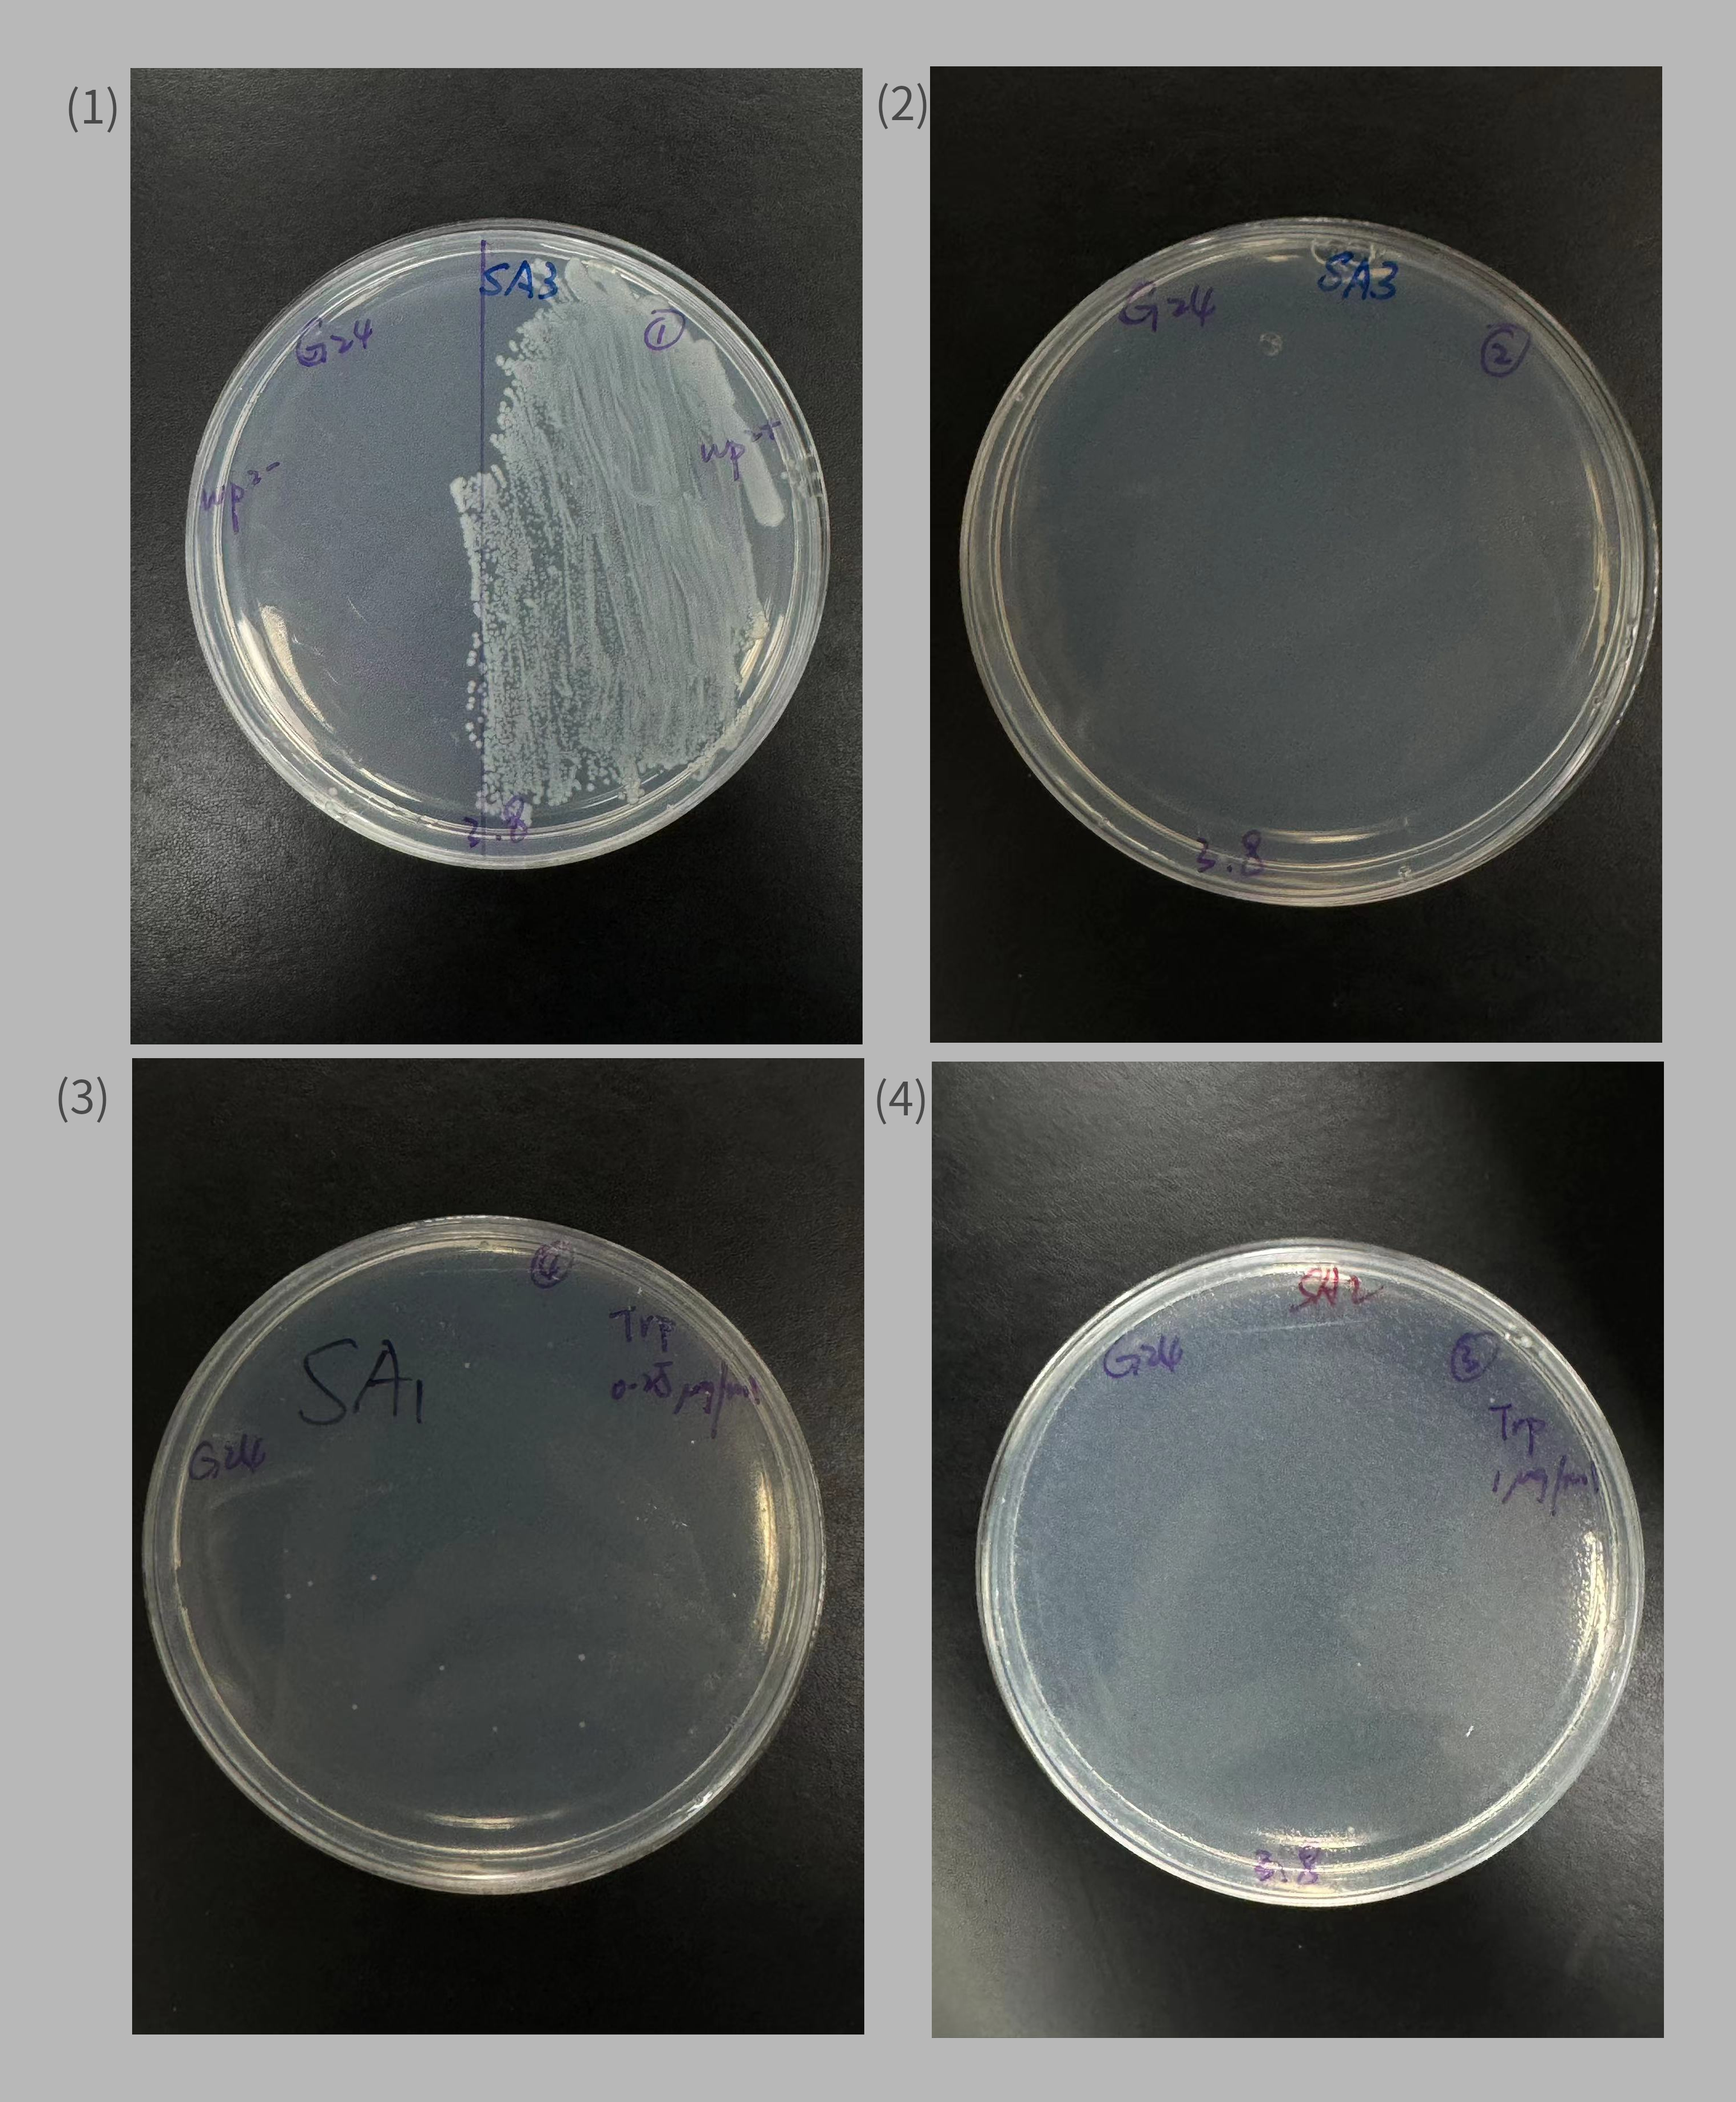
\includegraphics[width=0.48\textwidth]{1-4.png}
\caption{plate 1-4} \label{fig1}
\end{figure}


The results of plates 5 and 6 are shown in Figure 2. Both plates contained nutrient agar medium with sufficient tryptophan, expected to support the normal growth of tryptophan auxotrophic cells. These plates were designed with consecutive dilution factors of $10^5$ and $10^6$ to provide an appropriate range for counting colony-forming units (CFUs). However, as shown in Figure 2, plates 5 and 6 exhibited almost no visible colonies, contrary to expectations, making it impossible to calculate the colony concentration further. This discrepancy suggests that the absence of colonies was likely due to the omission of tryptophan in the agar medium preparation.


\begin{figure}[H]
\centering
\includegraphics[width=0.48\textwidth]{5-6.png}
\caption{plate 5 and plate 6} \label{fig2}
\end{figure}


Figure 3 illustrates the results of plates 7-10. The third group underwent chemical mutagenesis using MMS to assess mutagenicity in Escherichia coli. Two types of screening assays were conducted. For the spot test groups on plates 7-9, the water control (plate 9) was effective, as only 5 colonies were observed on the plate, representing spontaneous revertants from the spot test. Compared to spontaneous mutations, it is evident that the mutation frequency induced by MMS was much higher than the control group, with 32 colonies on plate 7 and 59 colonies on plate 8. Colonies in plates 7 and 8 were unevenly distributed. A clean circular inhibition zone was observed near the center spot, indicating the absence of colonies \cite{krishna2007uv}. Most colonies were located near the spot but did not invade it, and a few colonies were found at the edges of the plates.This phenomenon may indicate that revertants near the center may be dead, making the data less reliable. The number of revertants on plates treated with MMS was 15-30 times higher than that of spontaneous revertants. The difference in the number of revertants between 1\% and 2\% MMS solutions was approximately 2-fold, indicating a simple linear relationship between MMS concentration and WP2 revertant frequency.


\begin{figure}[H]
\centering
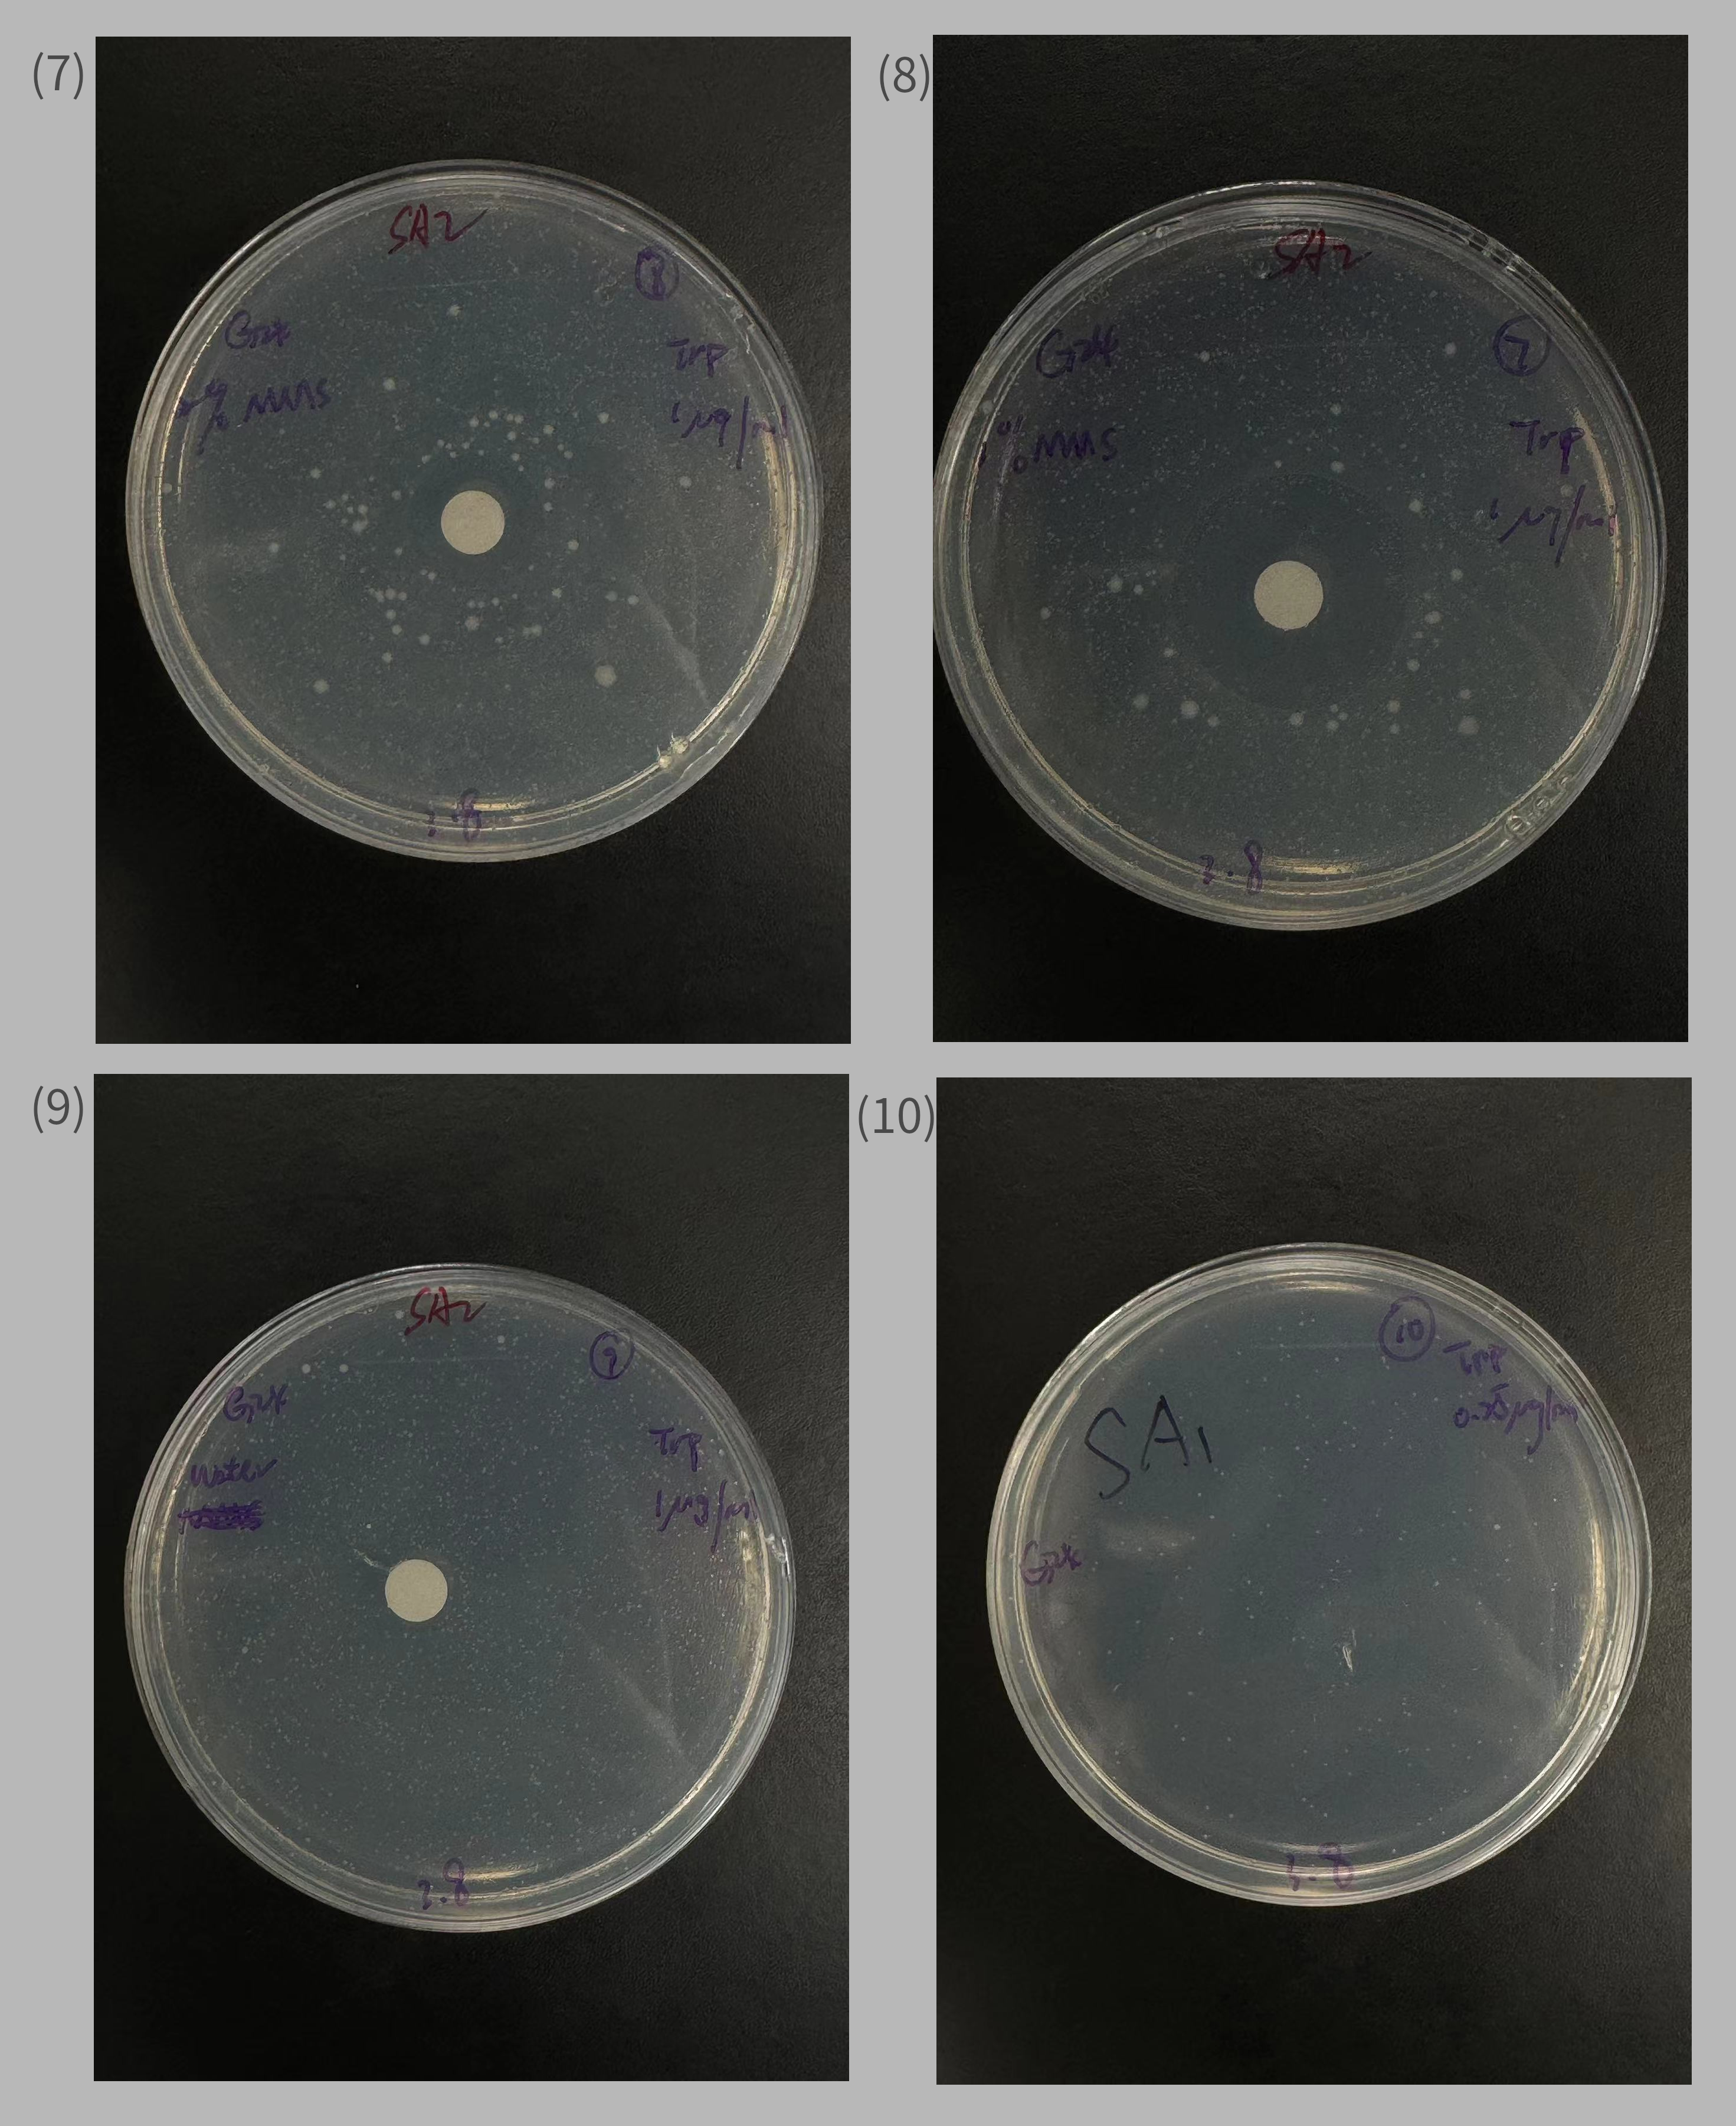
\includegraphics[width=0.48\textwidth]{7-10.png}
\caption{plate 7-10} \label{fig3}
\end{figure}


Regarding the plate incorporation test, plate 10 results showed only 2 colonies, similar to the results of spontaneous mutations. Theoretically, the plate incorporation test is more sensitive than the spot test because it allows the bacteria to be fully treated with the mutagen in the liquid suspension. However, the significantly lower number of colonies on plate 10 compared to plates 7 and 8 can be explained by the cytotoxic effects of MMS. When MMS induces bacterial mutations, it simultaneously kills many bacteria. Many induced revertants were likely killed before they could proliferate to form colonies \cite{grzesiuk1998role}. Finally, plates 11 and 12 (representing Group 4, used to explore the effects of UV light) yielded 7 and 3 colonies, respectively (Figure 4). It can be inferred that exposure to UV light for 20 seconds resulted in more viable revertants compared to exposure for 40 seconds.


\begin{figure}[H]
\centering
\includegraphics[width=0.48\textwidth]{11-12.png}
\caption{plate 11 and plate 12} \label{fig4}
\end{figure}


Due to the unexpected outcomes of plates 5 and 6, it was not possible to calculate the expected total number of viable cells. Referencing the data from Group 8 and Group 23, Table 4 was derived. It was observed that plates 5 and 6 in these two groups exhibited abundant colony growth. Using the data from Group 8, a series of calculations including CFUs were performed. The colony count on plate 6 was used to infer the assumed viable cells, with the countable range of colonies being between 30 and 300. Although the viable cells were assumed to have a value of $5.6\times10^8$ cfu/mL, the expected viable cells per treatment plate were $5.6\times10^7$ due to the 0.1 mL volume of culture material added to each plate. Plate 2 was used to estimate the spontaneous mutation frequency, which was calculated as $1.79\times10^{-8}$. This was because all observed single colonies on plate 2 originated from the $trp^+$ revertants in the bacterial culture before plating, whereas the corresponding plates for the other two groups were developed from both the original revertants and newly emerged revertants during the initial cell division phase.


\begin{center}
{\footnotesize Table 4. Statistics on the number of colonies in groups 8 and 23}
\vspace{0pt}
\begin{table}[H]
\setlength{\tabcolsep}{5pt}
\footnotesize
\begin{tabular}{ccccccccccccc}
\toprule [1pt]
Plates&1&2&3&4&5&6&7&8&9&10&11&12\\
\hline
G8&/&1&3&5&550&56&44&91&6&6&21&6\\
G23&/&2&12&3&680&142&48&70&2&5&3&48\\
\bottomrule [1pt]
\end{tabular}
\end{table}
\end{center}





\section{Discussion and Conclusion}


This study aimed to investigate the mutagenic effects of MMS and UV light on WP2 trp. The findings suggest that both MMS and UV light are mutagenic to E. coli auxotrophs, with mutation rates increasing with MMS concentration, albeit not in a linear fashion. Shorter UV light exposure periods favored reverse mutagenesis, while longer exposures resulted in fewer colonies. However, the mutagenic impact of MMS in the treat-and-plate test appeared to be masked by its cytotoxicity.

The logarithmic relationship between MMS dose and mutation frequency showed a positive linear correlation, consistent with previous research. For instance, the plate treated with 2\% MMS exhibited approximately twice as many revertant colonies as the plate treated with 1\% MMS, suggesting a possible positive correlation. However, due to the limited number of test groups with varying concentrations, a detailed understanding of this relationship was not achievable.

The overall conclusions regarding the mutagenic effects of both MMS and UV light are compelling, considering the differences in scales between spontaneous and induced mutation frequencies. Molecular rationale further supports these conclusions. MMS induces mutations by methylating purines, resulting in the formation of toxic non-canonicals that are excised to form apurinic sites for further base transversion. UV light induces mutations by forming base dimers and through the function of error-prone polymerase, supporting its mutagenic effects at the molecular level \cite{ikehata2011mechanisms}.

Prolonged UV exposure would kill too many bacteria to be detected, given UV light's disinfection function. However, defining what constitutes prolonged exposure is challenging. For instance, while 20 seconds of exposure may be suitable for inducing mutations, a 40-second period is not appropriate. The specific trends within the 20-second interval are not characterized. Therefore, additional experimental groups with smaller exposure intervals are required to comprehensively study UV mutagenesis.

The unexpected results of plate 10 can be attributed to the cytotoxicity of MMS, which decreases the survival ratio of WP2 with increasing MMS dose. The clear inhibition zone observed in the spot test plate further supports the toxicity of MMS \cite{green1976mutagen}.

\bibliographystyle{unsrt}
\bibliography{reference}

\end{multicols}

\includepdfmerge{question.pdf,1-5}
\includepdfmerge{evaluation.pdf}


\end{document}
